\documentclass[UTF8]{article}
\usepackage{ctex}
\usepackage{geometry}		%%页边距设置
\usepackage{booktabs}		%%排版表格
\usepackage{graphicx}
\usepackage{subfigure}	%%排版图片两个包

%\usepackage{lipsum}		%%乱序填充英文文字
%\usepackage{algorithmic}		%%这是代码的包
%\usepackage{indentfirst}  %%据说是自动首行缩进

\geometry{left=3cm} 
\geometry{right=2cm} 
\geometry{textheight=20cm}


\title{ The application of ML in the field of Network security}
\author{邵政道 \footnote{PB17061287,szd549845545@mail.ustc.edu.cn} \and 汪书畅 \footnote{PB17071369,wangsc014@mail.ustc.edu.cn}}

\renewcommand{\abstractname}{Abstract}
\renewcommand{\refname}{References}

\date{May.10th.2020}

\begin{document}

\maketitle{}

\begin{abstract}

	Machine Learning can deeply mine the value of big data, which is widely used in various fields. At the same time, it has related applications in the field of network security. For example, it has different applications in identity recognition and authentication, social engineering, network security, web security, security vulnerability and malicious code, intrusion detection and defense. This paper focuses on the application of machine learning in Cyberspace Security. And in the detection of attacks based on the destruction of network structure, the practice project of intrusion detection algorithm for KDD CUP99, the practice of spam recognition algorithm based on Ling spam dataset and naive Bayesian algorithm, the code practice is carried out, and the results are analyzed. At last, some prospects of machine learning in cyberspace security applications are put forward.

\end{abstract}

\section{Introduction}
	Machine Learning (ML) is a kind of data analysis method. It uses algorithms to build analysis model automatically. These algorithms can learn from data easily and automatically, and find the accuracy of data without using explicit programming.\cite{1} Machine learning integrates many fields of mathematics, including statistics, probability theory, linear algebra and mathematical calculation. The "training" and "prediction" processes in machine learning can correspond to the "induction" and "speculation" processes of human beings. Part of machine learning is shown in the figure below.
	
\begin{figure}[h]
\centering
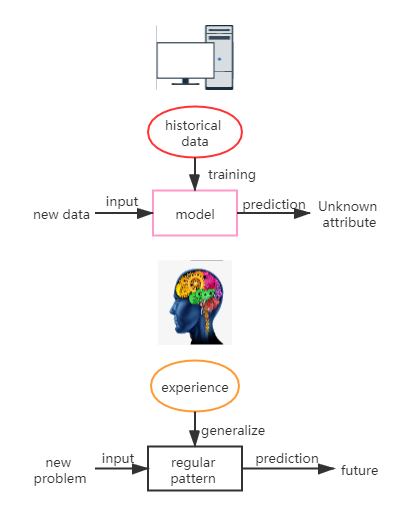
\includegraphics[scale = 0.5]{0}
\caption{The difference between machine learning and human brain}
\end{figure}
	
	Machine learning is a multi-disciplinary, its essence is to learn in data, through the appropriate algorithm modeling, and finally achieve classification, clustering or prediction in the case of no rules. In the machine learning evaluation of detection, clustering type is the most commonly used. \cite{5} Machine learning is often used in three directions: malicious code identification, social workers' security and intrusion detection.
	
\begin{itemize}
\item In terms of malicious code and malware identification

	Early detection of Internet of things malware network activities using machine learning technology. Check the features after the infected machine is infected and before the attack, and detect malicious activities in the scanning / infection stage. Because there must be a connection between the intruded machine and the attacker, at least there will be traffic that determines the moment of attack. \cite{Early Detection of IoT Malware Network Activity Using Machine Learning Techniques}Different from the traditional black-and-white list library, feature detection, heuristics and other methods of machine learning security applications from the anti-virus code classification, malicious file detection, malicious URL page code recognition and so on. For example, the machine learning method of malware detection based on apks can identify the disagree graph of Android malware, and different clustering and classification methods can be used to improve the detection ability of malware. This paper summarizes three kinds of malicious application recognition methods: match based detection, pattern based detection and learning based detection. \cite{State key laboratory of Computer Science, Institute of Software}Some reports, such as those from Macfee, say that about 3 million newly synthesized malicious files are generated every 60 minutes. The expected goal is that system learning will be the main target to eliminate the current attack scenario. \cite{Mayur Rele Cyber Security: Threat Detection Model based on Machine learning Algorithm}
	
\item	On social workers' security

Different from traditional technology and business experience analysis, security publicity, financial model and other evaluation methods, the security applications of machine learning range from harpoon phishing detection, malicious user click stream identification, fraud phone and SMS analysis, to financial credit fraud and so on.

\item  In Intrusion Detection

Different from the traditional rules and policies, regular matching and so on, machine learning security applications from DDoS Defense, webshell detection, DGA prevention to apt detection and so on. There is adaptive network security based on stream machine learning. Stream machine learning analysis includes processing one data instance at a time and checking only once. Therefore, limited memory is used. We evaluate the performance of two popular flow based machine learning algorithms. Hoeffding adaptive tree (HAT) and adaptive random forest (ARF). \cite{A Deep Learning Approach for Network Intrusion Detection System} It also uses nsl-kdd data set to discover the applicability of deep learning in NIDS implementation. \cite{5} The feature learning task of this method is completely unsupervised and based on sparse self coding. A deep learning method of network traffic recognition based on sparse self encoder is observed in \cite{Applications of Deep Learning on Traffic Identification}. In the work, the author realizes the unknown protocol recognition based on TCP instead of network intrusion detection.
	
\end{itemize}

	On the whole, even though machine learning is difficult to achieve 100\% correct effect after training the model, compared with the traditional means, the effect has been improved in varying degrees.
	



\section{Introduction to common open data sets in machine learning}

\subsection{KDD99 \cite{15}}

	Intrusion detection data set this data set is a 9-week network connection data collected from a simulated U.S. Air Force LAN, which is divided into labeled training data and unlabeled test data. Test data and training data have different probability distribution. The test data contains some attack types that do not appear in the training data, which makes the intrusion detection more realistic. In the training data set, there are 1 normal type and 22 training attack types, and 14 attacks only appear in the test data set.

\subsection{NSL KDD}
	Intrusion detection data set nsl-kdd data set solves the inherent problems in KDD99 data set. Due to the lack of public data set based on intrusion detection network, nsl-kdd data set still has some problems, and is not the perfect representative of the existing real network. But it can still be used as an effective benchmark data set to help researchers compare different intrusion detection methods. The setting of nsl-kdd training set and test set is reasonable, and the evaluation results of different research work will be consistent and comparable.
	

\subsection{NASA MDP}
	
	Software defect data set the NASA IV \& V facility metrics data program (MDP) data set published by NASA is widely used by the software defect prediction research center. MDP is an open data warehouse. The openness of the data set facilitates the repetition, improvement and even refutation of experiments by different researchers. The MDP consists of 13 different datasets, all from 13 actual NASA software projects, written in the most common development languages. Each dataset contains several modules from different software projects, ranging in size from 125 modules to 17186 modules. Each data set consists of several kinds of metric meta attributes, such as LOC, McCabe, Halstead, etc., and the defective ones. For the records provided by MDP data set, one row represents one module, and each field corresponds to one attribute.
	
	
\subsection{Ling-Spam dataset \cite{18}
\cite{19}}

This dataset is a small-scale preprocessing subset of the Ling spam dataset provided by ion androutsopoulos. The training and test data are stored in the format of TXT. It is based on 960 real emails from the linguistic mailing list. This email deleted some common words, converted all letters into lowercase, and deleted all numbers and punctuation to make the machine more efficient in identifying the content of the email.

\section{ Specific process of machine attack detection}

\subsection{The basic working steps of machine learning are as follows \cite{9}}

\begin{enumerate}

\item According to the training data (training model), the features are classified.

\item Classify the attribute set necessary for classification.

\item Model learning using training data (with ML algorithm).

\item The unknown data class is established by using the trained model, and the result is predicted.

\end{enumerate}

\subsection{Security problem abstraction of machine learning \cite{10}}

\begin{figure}[h]
\centering
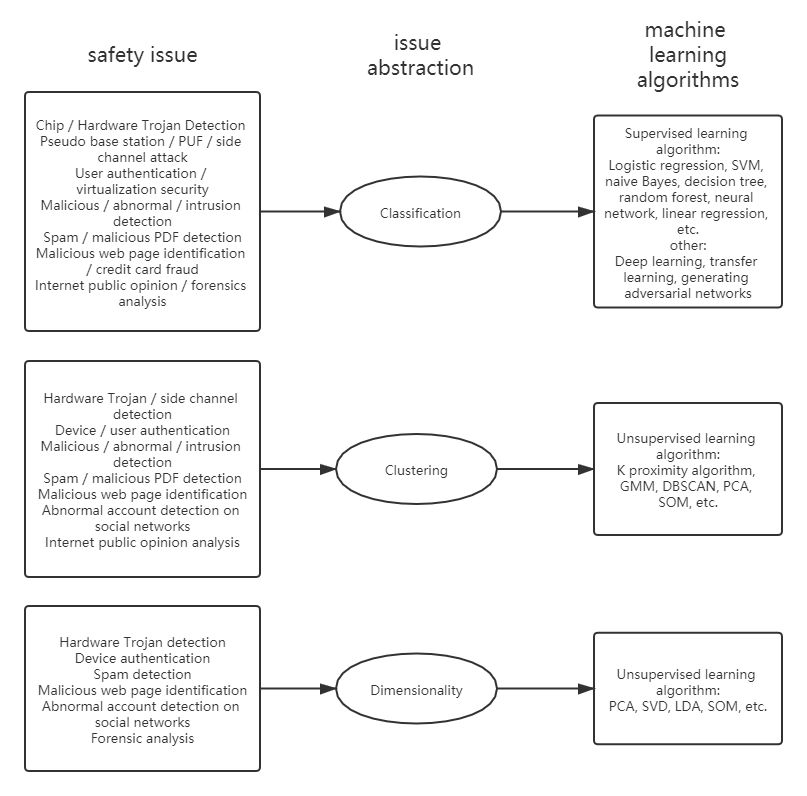
\includegraphics[scale = 0.5]{6}
\caption{Three types of machine learning}
\end{figure}

\subsection{Effectiveness evaluation index in security field \cite{10}}

\begin{center}

 \begin{tabular}{lcl}

  \toprule[2pt]
  
{\bfseries Evaluation indicators} & {\bfseries Describe} \\
  \midrule
TP(True Positive) & Number of samples correctly identified as normal \\
FN(False Negative) & Number of samples wrongly identified as malicious \\
FP(False Positive) & Number of samples incorrectly identified as normal\\
TN(True Negative) & Number of samples correctly identified as malicious \\


ACY(Accuracy) & Accuracy ACY=(TP+TN)/(TP+TN+FP+FN)\\
P(Precision) & Precision rate,P=TP/(TP+FP) \\
TPR(TP Rate) & True Positive Rate,TPR=TP/(TP+FN)\\
FPR(FP Rate) & False Positive Rate,FPR=FP/(FP+TN) \\
FNR(FN Rate) & False Negative Rate\\
  \bottomrule[2pt]
 \end{tabular}
\end{center}

\section{A case study of machine learning in Cyberspace Security}



\subsection{ Detect attacks based on network structure destruction }


Attacks based on the destruction of network structure will inevitably result in the change of network performance. How to detect this kind of attack and restore the normal operation of the network in the shortest time is the basis of preventing attacks on the network, which is to detect the defects in the network.\cite{13} Firstly, we introduce the machine learning detection method of related link failures, and carry out relevant practice.

The machine learning algorithm developed for link failure is divided into three stages. The first phase will detect if a link failure has occurred. If a link failure occurs, the second stage identifies whether a link reconnect and a link disconnect has occurred. Finally, the third stage locates a link failure, that is, the location of a disconnected or reconnected link. The author of this algorithm calls it (ml-lfil). The main idea of this algorithm is as follows:

\begin{itemize}
\item The passive monitoring method is used to identify and locate the link fault in the complex network.
	
\item	A machine learning model is developed, which can learn the traffic behavior under normal working conditions and different link failures.

\item  A te based machine learning technology is developed for link fault identification and location.

\item Two random complex networks and one network in Internet topology zoo are tested extensively to prove the effectiveness of the method.
	
\end{itemize}

\subsubsection{feature extraction}

The total transfer rate of the stream to other nodes in the network. We express BS, D as the total traffic from node s to node D.

The end-to-end delay d s, D, is the RTT delay of packets sent from node s to node D.

The packet loss rate expressed as LS, D is the ratio between the number of packets lost on the path between node s and node D and the total number of packets transmitted between two consecutive sampling instants.

Obviously, the decrease of the rate, or the increase of the delay and packet loss rate indicate the problem of a link to some extent. This is a relatively easy index, because in each network simulation platform, it can get feedback directly and in real time.

\subsubsection{Algorithmic idea}

Ml-lfil consists of three phases. Given the traffic information captured from the network, the first stage uses the link disconnection classifier to detect whether the link disconnection occurs.

Assuming that a link disconnect occurs, the second phase uses a delay regression to identify a link fault: only a link disconnect occurs, or a link disconnect and a link reconnect occurs. Finally, the third phase uses the link reconnect classifier to localize the link reconnect and correct the disconnect caused by the first phase.


\subsection{ Practical project of intrusion detection algorithm for KDD CUP99 }

\subsubsection{Project introduction}

In the practical part, due to the difficulty of direct replication algorithm, first of all, we find some relevant codes on GitHub \cite{14}, draw lessons from their codes, and design an algorithm for KDD CUP99 data set analysis based on our previous reading papers and understanding the idea of the algorithm.

As we know, the first 41 items of this data set are features, the 42nd item is tags, and the 41 features are divided into four categories:

\begin{enumerate}

\item Basic characteristics of TCP connection

\item Content characteristics of TCP connections

\item Statistical characteristics of network traffic based on time

\item Statistical characteristics of network traffic based on host

\end{enumerate}

KDD data set provides us with a very good reference. We have simplified the KDD data set itself, obtained the standardized and normalized small KDD data set by consulting some data, classified it by KNN algorithm, and drawn it by Python's Matplotlib package, and obtained the following results.

\begin{figure}[h]
\centering
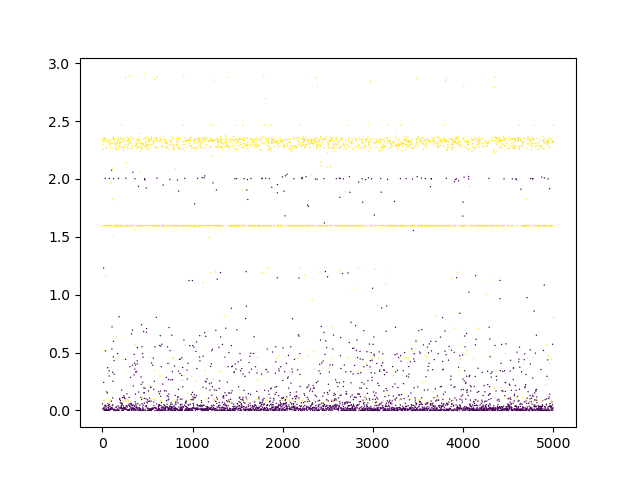
\includegraphics[scale = 0.5]{1}
\caption{Data security label category}
\end{figure}

The abscissa represents the serial number, the ordinate represents the classification score, and different colors represent different classifications. About 5000 information records have their own classifications. After listing, you can get the corresponding information security categories by comparison.

\subsubsection{KDD CUP99 algorithm instance running based on scikit learn tool}

In the example, we select the decision tree algorithm to detect POP3 brute force cracking, which is often referred to as password guessing. In KDD 99, there are columns 1, 5-9, 23-31. We chose the scikit learn tool.

Scikit learn (sklearn) is a common third-party module in machine learning. It encapsulates common machine learning methods, including regression, dimension reduction, classification, clustering and other methods. When we face the problem of machine learning, we can choose the corresponding method according to the figure below. Sklearn has the following characteristics: simple and efficient data mining and data analysis tools enable everyone to reuse and establish numpy, SciPy and Matplotlib in a complex environment. In the network attack, data classification is the main problem. In a large scale, it is a two classification problem, that is, security or insecurity. More detailed classification needs to identify more special attack methods.

On the official website of dataset \cite{15}, we obtained the corrected dataset specially prepared for verification, and carried out classification processing and training for it. The selected model is a decision tree. The output of the recognition results is as follows. The meaning of the matrix is the output of the cross ﹣ val ﹣ score function, that is, the score array of each run of cross validation. The specific meaning needs to be further understood, but from the numerical point of view, the accuracy is high.

\begin{figure}[h]
\centering
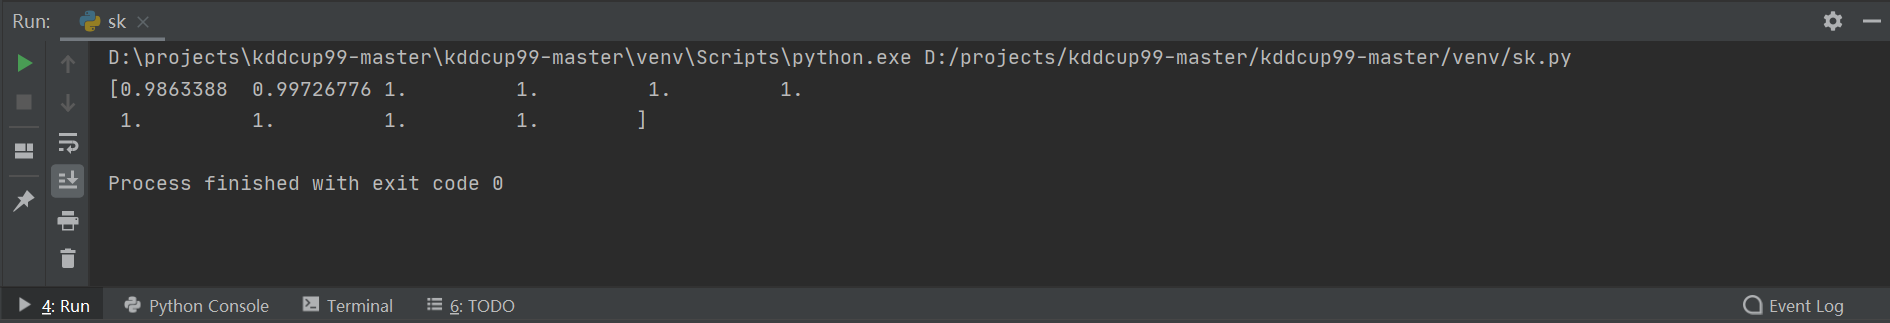
\includegraphics[scale = 0.3]{2}
\caption{Code run results}
\end{figure}

\subsubsection{Decision tree analysis results}

The analysis results of the decision tree are exported as follows according to pydotplus.graph "from" dot "data.

\begin{figure}[h]
\centering
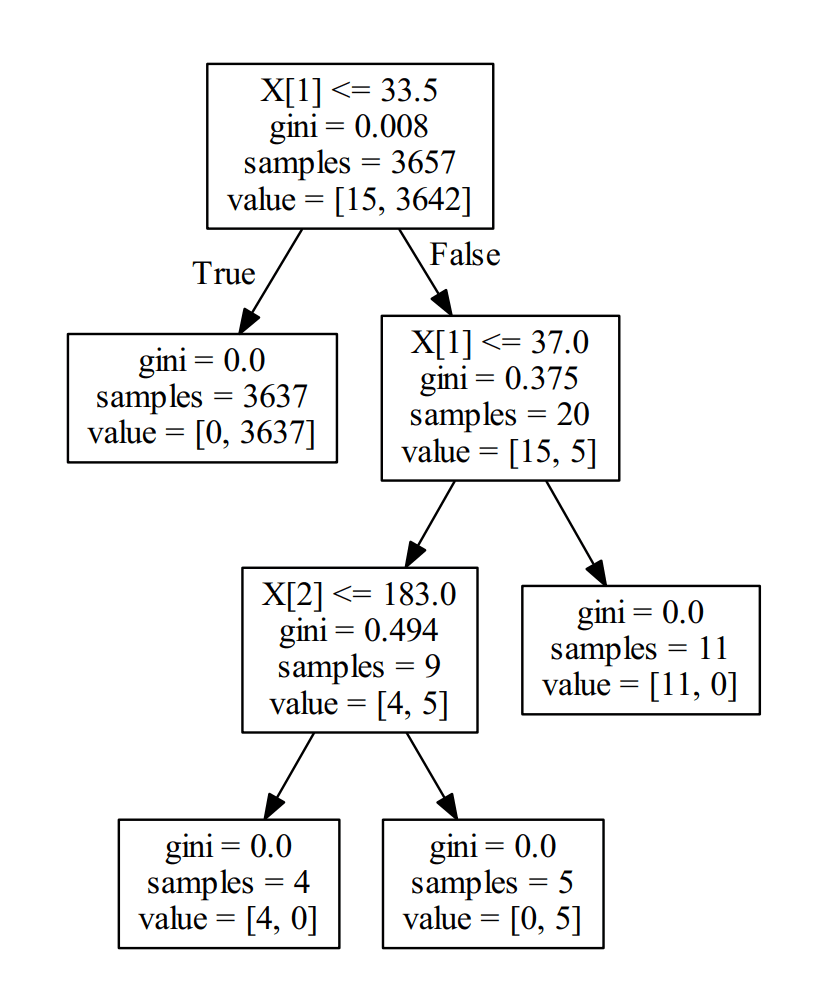
\includegraphics[scale = 0.2]{3}
\caption{Decision Tree}
\end{figure}

\subsubsection{Project summary}
We used some methods to perform some simple processing on the KDD CUP99 data set. The intrusion detection method is basically to design a classifier that can distinguish normal and abnormal data in the data stream, so as to alert the attack behavior. Generally, an analyst trains the classifier on 10\% of the training set in the data set, and then uses the corrected test set to test the performance of the classifier. This classifier can be Bayesian, decision tree, neural network, or SVM. The classification tool can be based on Scikit-learn or Tensorflow. After processing and training KDD CUP99, a classifier is obtained, and the data obtained in the actual situation can be classified. This is the significance of KDD CUP99 data set, which is an old one born over 20 years ago.

\subsection{Spam recognition algorithm based on Ling spam dataset and naive Bayesian algorithm}

\subsubsection{Data set introduction}

In the previous part, we have made some brief introduction to the Ling spam dataset, now we mainly introduce the content of the dataset. The Ling spam dataset contains 350 emails of "nonspam train" and "spam train", which are regarded as training sets. The "nonspam train" and "nonspam test" folders constitute a test set containing 130 spam messages and 130 non spam messages. The name of the message serves as a label for message identification, but it should be ignored before making a prediction. After making the prediction, you can use the correct label to check whether the classification is correct.

\subsubsection{Training method based on Naive Bayes}

Naive Bayesian algorithm is one of the most widely used classification algorithms.

Naive Bayes method is based on Bayes algorithm, which assumes that the attributes are independent of each other when the target value is given. That is to say, no attribute variable has a large proportion in the decision-making result, and no attribute variable has a small proportion in the decision-making result. Although this simplification method reduces the classification effect of Bayesian classification algorithm to a certain extent, it greatly simplifies the complexity of Bayesian method in practical application scenarios. This project uses the word frequency statistics of normal mail and spam, and classifies the mail types according to the word frequency of the mail content.

\subsubsection{Project operation results}

The evaluation index of the project is based on the effect evaluation index of the whole field mentioned before

\begin{figure}[h]
\centering
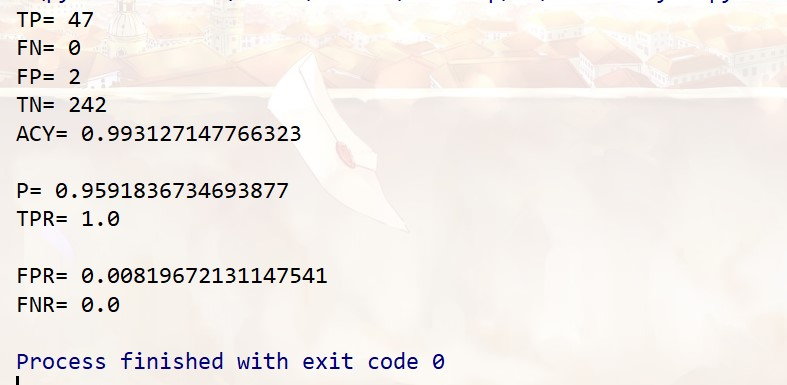
\includegraphics[scale = 0.5]{4}
\caption{Code run results2}
\end{figure}

\subsubsection{Result analysis}

According to the output results, the accuracy is 95.9\%, the recall rate is 100\%, the false alarm rate is 0.8\%, and the false alarm rate is 0\%. The training results show that the trained machine can distinguish the spam with high efficiency.

\subsubsection{Program block diagram}

\begin{figure}[h]
\centering
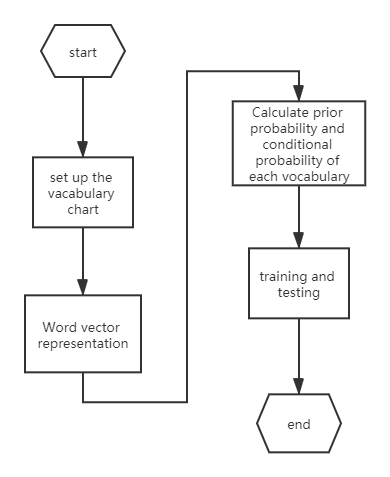
\includegraphics[scale = 0.4]{5}
\caption{Program block diagram}
\end{figure}

\section{Some new ideas}

At present, there are two keys to combine machine learning and network security: how to obtain meaningful data and how to develop effective algorithms.

\subsection{Summary of problems in data acquisition}

Data is the basis of machine learning, and the tools for data collection include Wireshark and other packet grabbing tools. However, the acquired data will have serious imbalance or noise problems due to various factors.

\subsubsection{Category imbalance}

In most cases, the number of packets with problems is far less than that without problems, which is the problem of class imbalance. Category imbalance refers to the great difference in the proportion of different categories of samples in the classification learning algorithm, which will cause significant interference to the learning process of the algorithm. At this time, we will use oversampling or undersampling to delete or increase the amount of data in some categories, which is reflected in the network security, i.e. deleting part of the normal packet data obtained, or allowing the abnormal packets to be retrieved. This needs to be handled in the process of bag grabbing.


\subsubsection{Noise}

The noise often comes from the abnormal data or the fault of feature extraction. In some cases, a certain network data (such as TCP / UDP type) is missing too much. At this time, we need to consider reducing the weight of this indicator, or directly deleting this feature to avoid polluting the integrity of the data. If there are few missing values, a variety of filling methods can be used. If there is an abnormal value, the data will be deleted directly, and then the filling algorithm will be used.

\subsection{Problem summary of developing algorithm}

Network topology can be abstracted as graph structure in data structure. For limited scale LAN, graph processing can be used. The weight can be determined synthetically according to the data extraction. For large-scale networks, the method of network topology simulation is no longer desirable. The best way is to use passive detection method to obtain network indicators. In the related work of our study, the innovation and breakthrough of the algorithm is not obvious. Most of the existing algorithms, including some very classical machine learning algorithms, are used. The development of new algorithms is more significant for the improvement of data processing performance than the improvement of accuracy. Taking the ml-lfil algorithm mentioned before as an example, compared with the Ping based method, it has no improvement in accuracy and shorter running time. For the future, we may be able to develop better algorithms, with improved accuracy and performance. We can even consider the popular deep learning algorithm, which can automatically extract features.


\section{Summary}
We find that KDDCUP99 data set is included in the sklearn module. After that, we will learn the related data processing knowledge, and do data preprocessing and normalization work for the data. A good command of machine learning ability will be of great help to our work.

In recent years, machine learning has made a series of remarkable achievements, especially in image recognition, speech recognition, automatic driving and so on. Because of its wide applicability, it also attracts more and more hackers and security technicians to develop and utilize it. This paper mainly introduces some common applications of machine learning in network security, related data sets, general implementation process of machine learning, and completes three projects of ml-lfil (detecting attacks based on destroying network structure), intrusion detection algorithm practice for KDD CUP99, spam recognition based on Ling spam dataset and naive Bayesian algorithm. It is believed that the application of machine learning in Cyberspace Security will be more and more extensive and effective.

\begin{thebibliography}{99}

\bibitem{1}Anoop Kumar Jain and Satyam Maheswari。Machine Learning (ML) Methods on Cyber Security. “Survey of Recent of Science and Technology​, vol. 10, no. 35, pp. 1-7, 2017.

\bibitem{Adaptive Network Security through Stream Machine Learning} Pavol Mulinka ,Pedro Casas. Adaptive Network Security through Stream Machine Learning. Publication:SIGCOMM '18: Proceedings of the ACM SIGCOMM 2018 Conference on Posters and DemosAugust 2018 Pages 4–5 https://doi.org/10.1145/3234200.3234246.

\bibitem{5}M. Zaman and C. Lung, "Evaluation of machine learning techniques for network intrusion detection", NOMS 2018 - 2018 IEEE/IFIP.

\bibitem{Early Detection of IoT Malware Network Activity Using Machine Learning Techniques}Ayush Kumar and Teng Joon Lim .EDIMA: Early Detection of IoT Malware Network Activity Using Machine Learning Techniques.arXiv:1906.09715v1 [cs.CR] 24 Jun 2019 .

\bibitem{Mayur Rele Cyber Security: Threat Detection Model based on Machine learning Algorithm}Kushal Rashmikant Dalal ,Mayur Rele Cyber Security: Threat Detection Model based on Machine learning Algorithm.


\bibitem{State key laboratory of Computer Science, Institute of Software}Chong WANG1,4, Chang-you ZHANG3,4 and Yong-ji WANG1,4* 1 State key laboratory of Computer Science, Institute of Software, Chinese Academy of Sciences, Beijng, 100190, China. 2 College of Electrical and Mechanical Engineering, National University of Science and Technology Islamabad, 44000, Pakistan. 3 Laboratory of parallel Software and Computational Science, Institute of Software。Machine Learning Approach for Malware Detection by Using APKs.

\bibitem{19}Congzheng Song, Thomas Ristenpart, Vitaly Shmatikov, “Machine Applied Sciences and Technology, ​Volume 3, ISSN: 0976-4828, Learning Models that Remember Too Much”, 22 Sep 2017,pp. 68 - 75, June 2012.

\bibitem{10}张蕾,崔勇,刘静,江勇,吴建平。机器学习在网络空间安全研究中的应用。计算机学报,清华大学计算机科学与技术系;北京邮电大学网络与交换技术国家重点实验室。2017。


\bibitem{A Deep Learning Approach for Network Intrusion Detection System}Quamar Niyaz, Weiqing Sun, Ahmad Y Javaid, and Mansoor Alam 。A Deep Learning Approach for Network Intrusion Detection System。 EAI Endorsed Trans. Security Safety.2015.

\bibitem{13}Srinikethan Madapuzi Srinivasan,Tram Truong-Huu,Mohan Gurusamy, Machine Learning-based Link Fault Identification and Localization in Complex Networks, 2018,10.1109/JIOT.2019.2908019.

\bibitem{14}https://github.com/gongyan200/kddcup99.git.

\bibitem{Applications of Deep Learning on Traffic Identification} Z. Wang, The Applications of Deep Learning on Traffic Identification." https://goo.gl/WouIM6. 

\bibitem{15}KDD Cup 99,http://kdd.ics.uci.edu/databases/kddcup99/kddcup99.html.


\bibitem{18} http://www.aueb.gr/users/ion/data/lingspam\_public.tar.gz.

\bibitem{19}I. Androutsopoulos, J. Koutsias, K.V. Chandrinos, George Paliouras,  and C.D. Spyropoulos, "An Evaluation of Naive Bayesian Anti-Spam Filtering". In Potamias, G., Moustakis, V. and van Someren, M. (Eds.), Proceedings of the Workshop on Machine Learning in the New Information Age, 11th  European Conference on Machine Learning (ECML 2000), Barcelona, Spain, pp. 9-17, 2000.


\end{thebibliography}

\end{document}






























